\documentclass[conference]{IEEEtran}
\usepackage[T1]{fontenc}
\usepackage{newtxtext,newtxmath}  % IEEE house face; also keeps Type 1 outlines, not Type 3
\let\Bbbk\relax  % newtxmath already defines it; without this amssymb raises a LaTeX error
\usepackage{booktabs,graphicx,amsmath,amssymb,microtype,xcolor}
\usepackage{enumitem}
\usepackage[hidelinks]{hyperref}
% IEEEtranN.bst is the natbib-aware IEEE style, so \citep survives the template change.
\usepackage[numbers,sort&compress]{natbib}
\newtheorem{proposition}{Proposition}
\setlength{\textfloatsep}{8pt plus 2pt minus 2pt}
\setlength{\dblfloatsep}{6pt plus 2pt minus 2pt}
\setlength{\dbltextfloatsep}{8pt plus 2pt minus 2pt}
\newcommand{\nInterviews}{526}
\newcommand{\nSegments}{13,315}
\newcommand{\nNarrators}{470}
\newcommand{\nTranscripts}{519}
\newcommand{\labelCoverage}{77.7\%}
\newcommand{\nTurns}{220,471}
\newcommand{\turnAccuracy}{0.806}
\newcommand{\charsRemoved}{13.2\%}
\newcommand{\nRankTerms}{211}
\newcommand{\alphaRankTwo}{0.039}
\newcommand{\alphaRankOne}{0.073}
\newcommand{\alphaHead}{0.059}
\newcommand{\alphaTail}{0.037}
\newcommand{\rawAgreement}{0.530}
\newcommand{\gwetAC}{0.082}
\newcommand{\deferLexical}{46.0\%}
\newcommand{\deferBoth}{0.0\%}
\newcommand{\nDisputed}{146}
\newcommand{\leaFone}{0.196}
\newcommand{\leaThreshold}{0.60}
\newcommand{\rhoMerge}{84.1\%}
\newcommand{\rhoSplit}{81.0\%}
\newcommand{\extractorCorr}{0.451}
\newcommand{\falseSingleton}{0.367}
\newcommand{\nAmbiguous}{21}
\newcommand{\nExtractedEvents}{199}
\newcommand{\starLossless}{yes}
\newcommand{\nCells}{13,996}
\newcommand{\spearmanRho}{0.471}
\newcommand{\inversionRate}{1.0\%}
\newcommand{\concordanceRate}{81.4\%}
\newcommand{\invTwoThree}{37.1\%}
\newcommand{\rhoTwoThree}{0.169}
\newcommand{\pairsTwoThree}{9,870}
\newcommand{\largestRankTwo}{106}
\newcommand{\smallestRankThree}{1}
\newcommand{\largestRankThree}{157}
\newcommand{\sizeOnlyN}{211}
\newcommand{\sizeOnlyTree}{0.500}
\newcommand{\sizeOnlyLogit}{0.511}
\newcommand{\sizeOnlyPrior}{0.500}
\newcommand{\sizeOnlyMI}{0.000}
\newcommand{\sizeOnlyMax}{0.611}
\newcommand{\sfNarrTouched}{266}
\newcommand{\sfMeanRemoved}{13.8\%}
\newcommand{\sfLiftFiveGlobal}{0.268}
\newcommand{\sfLiftFiveSF}{0.306}
\newcommand{\sfLiftThreeGlobal}{0.165}
\newcommand{\sfLiftThreeSF}{0.163}
\newcommand{\sfMthreeMatched}{0.064}
\newcommand{\sfMthreeStrong}{0.139}
\newcommand{\sfMfive}{0.098}
\newcommand{\didPoint}{0.295}
\newcommand{\didLo}{0.258}
\newcommand{\didHi}{0.331}
\newcommand{\didNarrators}{188}
\newcommand{\rboCoarseMid}{0.537}
\newcommand{\rboCoarseFine}{0.251}
\newcommand{\rboMidFine}{0.317}
\newcommand{\rboThreshold}{0.60}
\newcommand{\interactionCoef}{-0.085}
\newcommand{\interactionP}{2.5 \times 10^{-17}}
\newcommand{\interactionCiLo}{-0.104}
\newcommand{\interactionCiHi}{-0.065}
\newcommand{\interactionNarrators}{445}
\newcommand{\interactionEvents}{75}
\newcommand{\interactionCoefOld}{-0.085}
\newcommand{\interactionEventsOld}{75}
\newcommand{\designEffect}{139.0}
\newcommand{\iccNarrator}{0.169}
\newcommand{\nClusters}{470}
\newcommand{\nIncidences}{383,680}
\newcommand{\ccnnAccPoint}{0.517}
\newcommand{\ccnnAccLo}{0.499}
\newcommand{\ccnnAccHi}{0.536}
\newcommand{\asoBonferroni}{110}
\newcommand{\asoConfidence}{1.000}
\newcommand{\segmentsWithTopics}{4,600}
\newcommand{\medianSegments}{23}
\newcommand{\pertRbo}{0.324}
\newcommand{\nRankTwoCells}{141}
\newcommand{\pertRboArchive}{0.978}
\newcommand{\pertThreshold}{0.70}
\newcommand{\pertPasses}{no}
\newcommand{\pertGridPoints}{25}
\newcommand{\extractorMinRbo}{0.251}
\newcommand{\goldSubsetSegments}{4,538}
\newcommand{\goldTermsExcluded}{21}
\newcommand{\goldCells}{127}
\newcommand{\goldMthree}{0.127}
\newcommand{\goldMfive}{0.091}
\newcommand{\goldMone}{0.132}
\newcommand{\singletonNarrators}{0.206}
\newcommand{\singletonWithInterviewers}{0.000}
\newcommand{\interviewerRbo}{0.882}
\newcommand{\triageK}{50}
\newcommand{\triageUnstable}{8}
\newcommand{\freqSpearman}{0.879}
\newcommand{\freqRbo}{0.444}
\newcommand{\freqJaccard}{0.500}
\newcommand{\transferSegments}{874}
\newcommand{\transferInterviews}{55}
\newcommand{\transferAlpha}{0.062}
\newcommand{\transferAlphaDrop}{-0.023}
\newcommand{\transferRho}{0.457}
\newcommand{\transferCells}{32}
\newcommand{\transferMthree}{0.356}
\newcommand{\transferMfive}{0.347}
\newcommand{\conclusionTransfers}{no}
\newcommand{\topoPermP}{1.000}
\newcommand{\topoBetaOneP}{1.000}
\newcommand{\topoBetaOneNullStd}{0.0}
\newcommand{\topoBetaZeroNullStd}{0.0}
\newcommand{\topoBetaOneRtwo}{0.998}
\newcommand{\topoFiltrationLevels}{25}
\newcommand{\topoKeep}{no}
\newcommand{\topoRedundant}{yes}
\newcommand{\convSubset}{200}
\newcommand{\convLossFive}{0.000}
\newcommand{\convValFiveFirst}{0.472}
\newcommand{\convValFiveLast}{0.503}
\newcommand{\convValFiveMax}{0.545}
\newcommand{\convEpochs}{600}
\newcommand{\liftConfigs}{9}
\newcommand{\liftExpLo}{0.599}
\newcommand{\liftExpHi}{0.735}
\newcommand{\liftSingLo}{0.140}
\newcommand{\liftSingHi}{0.654}
\newcommand{\selDisjAuc}{-0.050}
\newcommand{\selDisjMap}{-0.061}
\newcommand{\selRandAuc}{0.239}
\newcommand{\selRandMap}{0.236}
\newcommand{\selThreeMap}{0.162}
\newcommand{\selFiveMap}{0.102}
\newcommand{\selThreeEpAuc}{1.8}
\newcommand{\selThreeEpMap}{55}
\newcommand{\tuneFiveAuc}{0.568}
\newcommand{\tuneGap}{-0.050}
\newcommand{\tuneThreeLr}{0.005}
\newcommand{\tuneThreeDo}{0.1}
\newcommand{\facThreePlain}{0.065}
\newcommand{\facThreeEnc}{0.147}
\newcommand{\facFivePlain}{0.097}
\newcommand{\facFiveEnc}{0.101}
\newcommand{\facFiveEncAuc}{0.704}
\newcommand{\facFivePlainAuc}{0.550}
\newcommand{\facOpPlainDisj}{0.033}
\newcommand{\facOpPlainRand}{0.153}
\newcommand{\facOpEncDisj}{-0.046}
\newcommand{\facOpEncRand}{-0.041}
\newcommand{\facThreePlainLo}{0.049}
\newcommand{\facThreePlainHi}{0.081}
\newcommand{\facFivePlainLo}{0.074}
\newcommand{\facFivePlainHi}{0.122}
\newcommand{\costBuild}{0.23}
\newcommand{\costStar}{0.20}
\newcommand{\costFeat}{0.66}
\newcommand{\costTrain}{10.7}
\newcommand{\costGpu}{251}
\newcommand{\gapRealFive}{0.290}
\newcommand{\gapAnonFive}{-0.006}
\newcommand{\gapReductionFive}{0.296}
\newcommand{\gapRealThree}{-0.033}
\newcommand{\gapAnonThree}{-0.165}
\newcommand{\anonFiveRandom}{0.060}
\newcommand{\anonFiveNarr}{0.066}
\newcommand{\doseSlope}{0.015}
\newcommand{\doseSlopeLo}{-0.010}
\newcommand{\doseSlopeHi}{0.040}
\newcommand{\doseSlopeP}{0.22}
\newcommand{\doseNarrators}{447}
\newcommand{\doseSlopeControl}{-0.169}
\newcommand{\featGapMean}{0.315}
\newcommand{\featGapItem}{0.385}
\newcommand{\featGapMeanThree}{-0.024}
\newcommand{\featGapItemThree}{-0.018}
\newcommand{\exposurePredicted}{64.1\%}
\newcommand{\exposureSingletonN}{68}
\newcommand{\obsGround}{470}
\newcommand{\obsCells}{13,315}
\newcommand{\obsDistinct}{455}
\newcommand{\obsSingletonSupports}{441}
\newcommand{\obsMultiSupports}{14}
\newcommand{\obsCollapse}{29.3}
\newcommand{\obsMaxMult}{142}
\newcommand{\obsDesignCells}{9}
\newcommand{\straddleRandom}{64.8\%}
\newcommand{\straddleRandomN}{249}
\newcommand{\straddleEvent}{61.2\%}
\newcommand{\straddleEventN}{235}
\newcommand{\straddleTotal}{384}
\newcommand{\citationsVerified}{27}
\newcommand{\citationsTotal}{28}
\newcommand{\facExpFivePlain}{0.297}
\newcommand{\facExpFiveEnc}{-0.025}
\newcommand{\facExpThreePlain}{0.177}
\newcommand{\facExpThreeEnc}{-0.031}
\newcommand{\tuneFiveBest}{0.103}
\newcommand{\tuneThreeWorst}{0.133}
\newcommand{\tuneTrials}{8}
\newcommand{\facSeeds}{5}
\newcommand{\selSeeds}{5}
\newcommand{\tuneSeeds}{3}
\newcommand{\ablationNoMomentsTwo}{0.840}
\newcommand{\MthreeTone}{0.139}
\newcommand{\MthreeTtwo}{0.816}
\newcommand{\MfiveTone}{0.098}
\newcommand{\MfiveTtwo}{0.546}
\newcommand{\MoneTone}{0.069}
\newcommand{\MoneTtwo}{0.725}
\newcommand{\MzeroTone}{0.009}
\newcommand{\MzeroTtwo}{0.552}
\newcommand{\MfourTone}{0.012}
\newcommand{\MfourTtwo}{0.853}
\newcommand{\paramSpread}{2.8\%}
\newcommand{\nSeeds}{10}
\newcommand{\nTOneQueries}{400}
\newcommand{\paramBudget}{132{,}219}
\newcommand{\MthreeToneRandom}{0.106}
\newcommand{\MfiveToneRandom}{0.388}
\newcommand{\MthreeToneEvent}{0.033}
\newcommand{\MfiveToneEvent}{0.152}
\newcommand{\probeInputControl}{1.000}
\newcommand{\probeNarrThree}{0.862}
\newcommand{\probeChance}{0.011}
\newcommand{\probeClasses}{440}
\newcommand{\probeN}{12{,}846}
\newcommand{\probeNarrFive}{0.902}
\newcommand{\probeRandThree}{0.920}
\newcommand{\probeRandFive}{0.950}
\newcommand{\deffSqrt}{12}
\newcommand{\asoThreeOverFive}{0.00}
\newcommand{\asoFiveOverThree}{1.00}
\newcommand{\invarianceWins}{9}
\newcommand{\invarianceTotal}{11}
\newcommand{\buildDate}{2026-08-19}


\title{CAIRN: Ownership Obstruction and Evaluation Design
in Higher-Order Models of Oral History}
\author{\IEEEauthorblockN{Zeyu Dong and Roy Choi}
\IEEEauthorblockA{\textit{Independent Researcher}, Toronto, Canada \\
Correspondence: dongzeyu123@outlook.com}}
\newcommand{\repoURL}{https://github.com/AlexDongzeyu/CARIN}

\begin{document}
\maketitle

\begin{abstract}
A rank ladder is an information granulation, and combinatorial complexes make one
computable, with a growing family
of topological networks passing messages along
it~\citep{hajij2023tdl,papillon2023architectures}. Networks in that family act on cells, each
a subset of a ground set, so where that set holds entities and the items above them are
singly owned, two items with one owner are one cell. Singly owned items are what an
oral-history archive holds: across \nInterviews{}
interviews, \obsCells{} described moments realise \obsDistinct{} supports over
\obsGround{} narrators, so no combinatorial complex over those narrators holds them apart, a
collapse we call the \emph{ownership obstruction}. Lifting from rank 0
carries it into the
features: at most \obsDistinct{} distinct rank-1 inputs, a \obsCollapse{}-fold collapse. The
split
decides whether the collapse is visible. \straddleRandom{} of narrators straddle a random
split, a rate the entity-degree distribution predicts at \exposurePredicted{} before any
model exists. Given that exposure, a complex network appears to beat a lossless typed-star
expansion \MfiveToneRandom{} to \MthreeToneRandom{} in T1 MAP, and trails it \MfiveTone{} to
\MthreeTone{} once narrators are held out, while destroying entity identity removes the
complex's gain. Gains of that kind track the inputs rather than the operator: the star leads as
registered, carrying spectral encodings the complex never receives, the ordering reverses
once both read the same features, and on those matched inputs both architectures leak,
\facExpFivePlain{} against \facExpThreePlain{}.
Assigning the middle rank is itself underdetermined, three programmatic operationalisations
of one written manual agreeing at $\alpha = \alphaRankTwo{}$. What is new is the combination:
an injectivity test that runs before training, an exposure rate predicted in closed form, and
a controlled ranking reversal inside an owner-grounded
hierarchy. The magnitude of the reversal is a finding about this archive; the obstruction
itself is structural, and reaches any collection whose items are singly owned.\footnote{Data,
code and audit record: \url{\repoURL}.}
\end{abstract}

\begin{IEEEkeywords}
information granulation, granular computing, topological deep learning, higher-order
networks, evaluation design, data leakage, oral history archives
\end{IEEEkeywords}

\section{Introduction}

A combinatorial complex assigns each cell a rank, so that each rank holds a coarser
information granule than the one below, and lets messages travel between ranks
as well as within them. Across those ranks, the operator family is rank-aware in a way graph
and hypergraph message passing is not, and the accompanying networks are designed to exploit
that~\citep{hajij2023tdl,papillon2023architectures}. For an archive, the appeal of such
networks is immediate, because testimony has obvious levels: a narrator, a moment inside an
interview, an event that several narrators describe, a longer episode that contains those
events. Those levels are tempting to read as a rank ladder, and reading them that way meets a
counting problem (Figure~\ref{fig:overview}): a combinatorial complex identifies a
cell with the ground elements it contains, so two moments told by one narrator are one cell,
and this archive's \obsCells{} moments carry \obsDistinct{} distinct supports over
\obsGround{} narrators. Those collapsed supports are what we call the \emph{ownership
obstruction}.

Before a rank-structured model can be said to help, three things have to be true.

\begin{description}[leftmargin=0em,itemsep=1pt,topsep=2pt,parsep=0pt]
\item[P1. Rank carries information beyond size.] Coarsening a partition ordinarily produces
larger blocks, so rank and size are expected to move together in any granulation. What a
curated ladder has to add to any granulation is the residual: if rank is recoverable from
cell size alone, the
ladder is a sorting of set sizes and nothing is gained by calling it structure.
\item[P2. The specification is stable.] If faithful independent implementations of the
same written manual assign a term to different ranks, the ladder cannot be operationalised
from the manual alone, and what fills the gap is the judgement of whoever built it.
\item[P3. The structure pays.] If a typed star expansion matches a full complex at equal
parameter count, the complex has not earned its additional structure.
\end{description}

We fixed thresholds and failure outcomes for all three before looking at any model result.
Against them, on an archive of \nInterviews{} interviews and \nSegments{} described segments,
\textbf{rank carries information beyond size, the specification moves when it is applied
twice, and the typed star beats the complex at equal parameter count}. The induced
partition moves under a defensible change of granularity as well, and the star's margin comes
from its inputs: on matched features the ordering reverses. That ladder is real; the
machinery built on it has still to earn its place.

A fourth result, undeclared in advance, matters most and concerns the train/test split.
Under a random split the ordering of architectures reverses and the complex's advantage is
large, while it leads under no other design axis we varied, which places that advantage in
the split rather than in the operator.

The reason lies in the feature construction these models are normally given. A
cell's features are aggregated from its constituent rank-0 narrators, and nearly every moment
has a single narrator, so such a moment's input vector \emph{is} its narrator's vector, and
two such moments land on both sides of a random split as the same vector. Shuffling
narrator identity removes that vector's privilege and with it the complex's entire
random-split advantage, while replacing the moment features with passage-specific text does
not, which locates the leak in the narrator layer. Those extra ranks buy a shorter path to
who is speaking.

Three things are new here. First, an exact support-injectivity test decidable on the
encoding before a model exists, where the surrounding literature offers diagnostics that
correlate with downstream behaviour. Second, an entity-exposure rate the degree distribution
predicts in closed form, so the leak is quantifiable from the data alone.
Third, a controlled reversal of the architecture ranking inside an owner-grounded
hierarchy, with the mechanism named and intervened on. All three describe an encoding and a
precondition on it, one level below the architecture comparisons they constrain.

\begin{figure*}[t]\centering
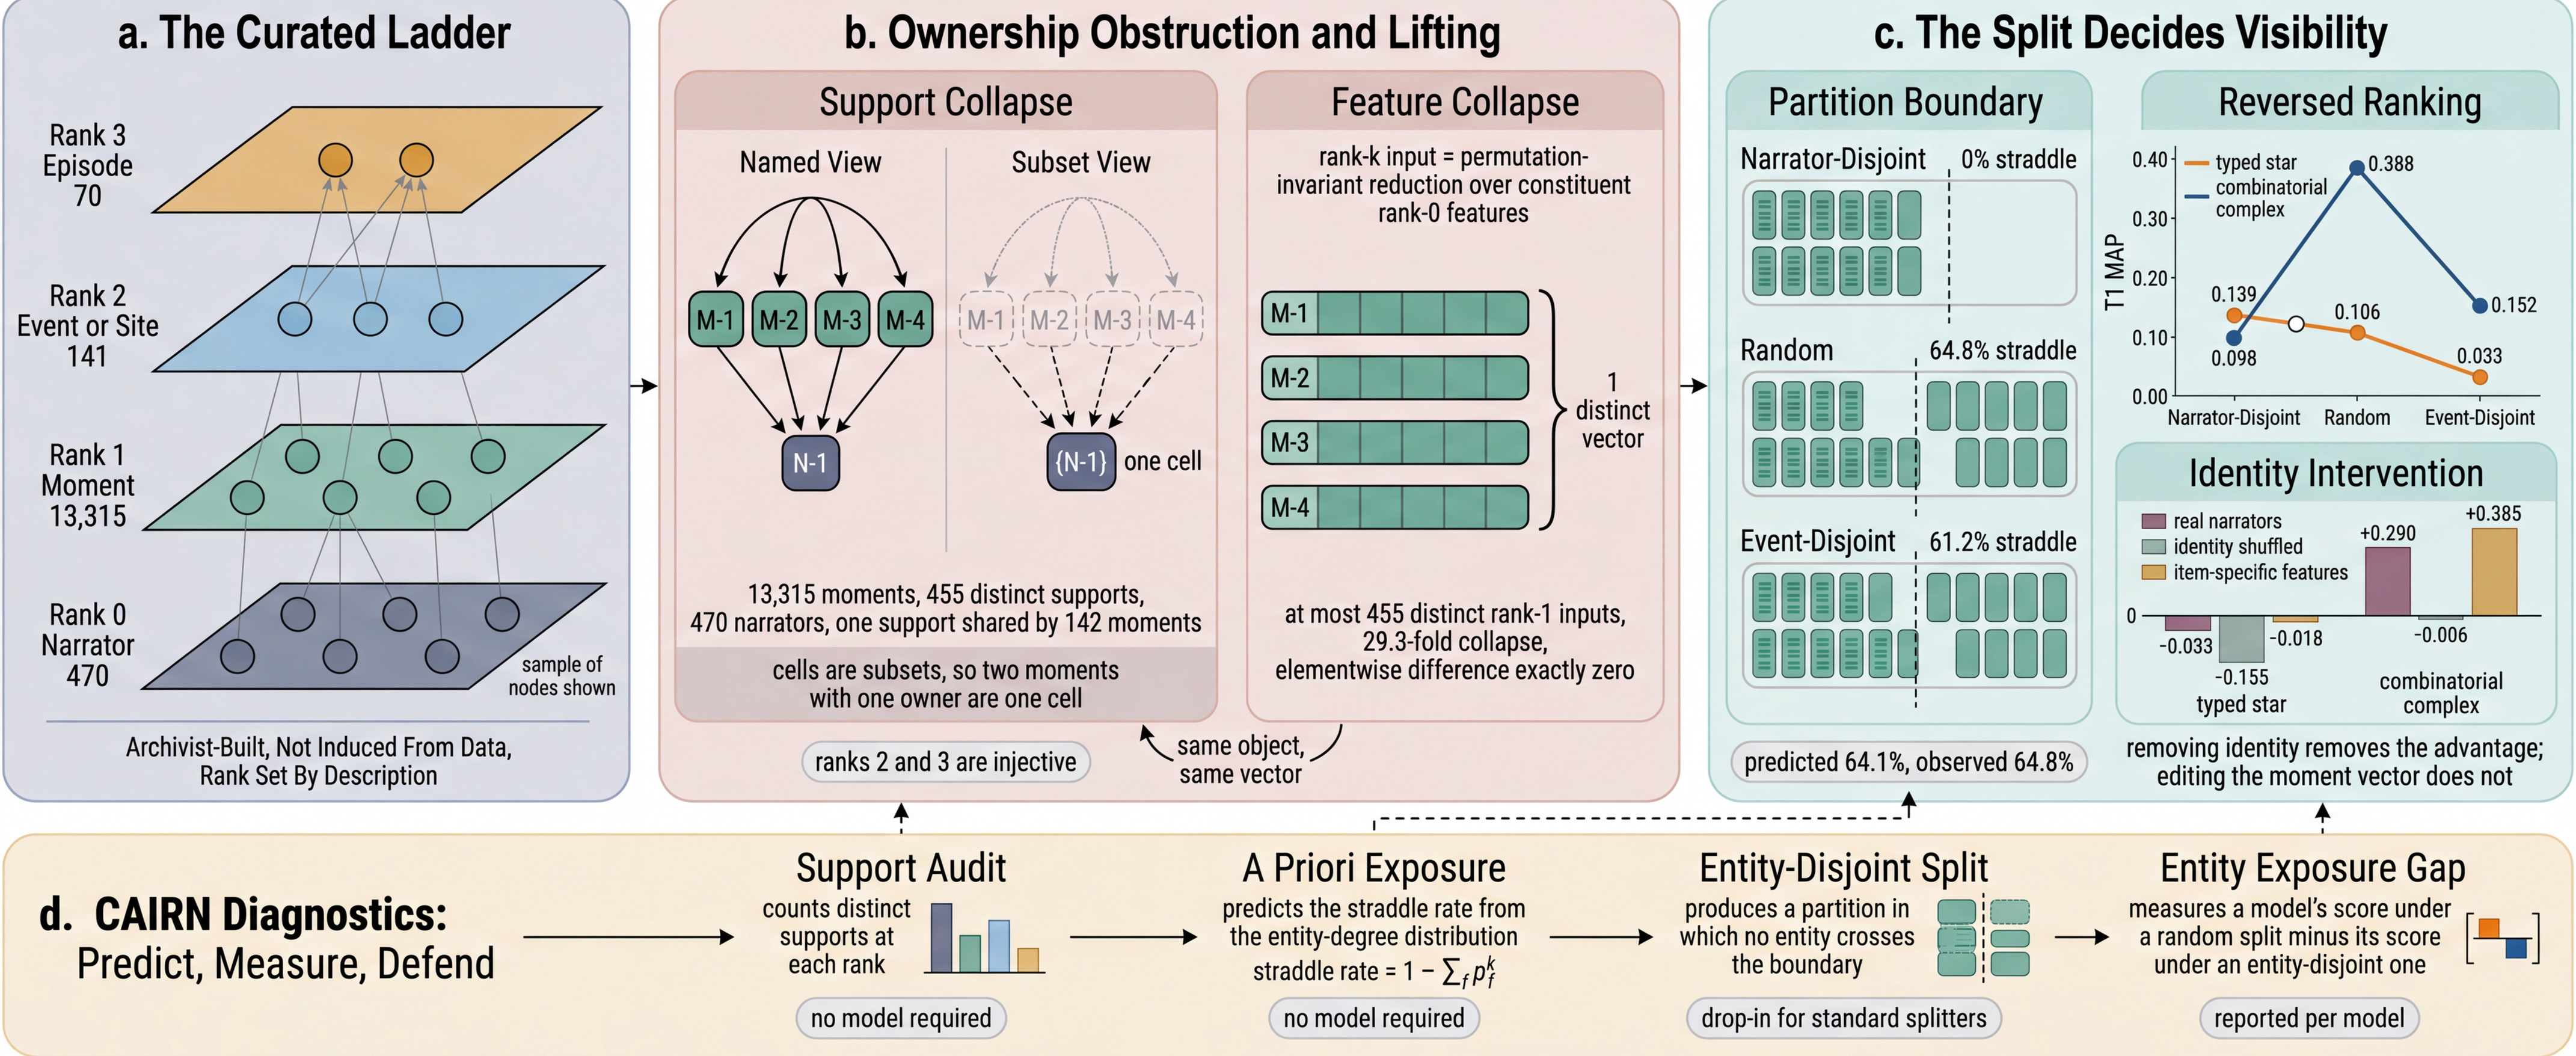
\includegraphics[width=0.74\textwidth]{../figures/fig1_overview.jpg}
\caption{The ownership obstruction and what it does to evaluation. \textbf{a}, The archive's
four-level descriptive ladder; node counts are illustrative, tier counts exact.
\textbf{b}, Rank-1 moments are almost all singly owned, so as subsets they are
indistinguishable: \obsCells{} moments realise \obsDistinct{} supports over \obsGround{}
narrators, leaving at most \obsDistinct{} distinct rank-1 inputs after lifting.
\textbf{c}, Whether the collapse is visible depends on the partition. Straddle rate is the
fraction of narrators on both sides; the predicted rate follows from the entity-degree
distribution alone, with $p_f$ the proportion of fold $f$ and $k$ the cells an entity owns.
T1 MAP reverses under a random split, and shuffling narrator identity removes the
complex's gain while the star's, never positive, falls further. \textbf{d}, The released
diagnostics; the first two require no trained model.}
\label{fig:overview}\end{figure*}

\section{Archive and rank ladder}

Our corpus is the Densho Digital Repository's Japanese American oral-history collection:
\nInterviews{} interviews
covering \nNarrators{} narrators, \nSegments{} segments carrying archival description, and
\nTranscripts{} transcripts, at a median of \medianSegments{} segments per interview. A
segment enters the event ranks only if it carries a topic term, which \segmentsWithTopics{}
of them do. Those ranks are taken from the archive's own
descriptive practice: rank 0 a narrator, rank 1 a
described moment within an interview, rank 2 an event or site, rank 3 the episode containing
it.

That ladder cannot be a combinatorial complex over the narrators, and the reason is
counting.

\begin{proposition}[Ownership obstruction]
\label{prop:obstruction}
Let $S$ be a ground set and let a collection $C_1$ carry a support map
$\mathrm{supp}: C_1 \to \mathcal{P}(S)\setminus\{\emptyset\}$. The cells of a combinatorial
complex over $S$ are subsets of $S$, so any two cells with the same support are the same
cell. If $C_1$ realises fewer than $|C_1|$ distinct supports then $\mathrm{supp}$ is not
injective, and no combinatorial complex over $S$ carries $C_1$ as distinct cells. Where every
cell has a single owner in $S$, that happens as soon as $|C_1| > |S|$.
\end{proposition}

The archive meets the condition at rank 1 (Figure~\ref{fig:overview}b). Over \obsGround{}
narrators at that rank, \obsCells{} described
moments realise \obsDistinct{} distinct supports, one of them shared by \obsMaxMult{} moments,
and the counts repeat in all \obsDesignCells{} design cells of the sweep because rank-1 cells
are the archive's segments. Among those supports, \obsSingletonSupports{} name single
narrators,
which is what holds the cell count below \obsGround{}, and the remaining \obsMultiSupports{}
are
the sets of two to four speakers who share a segment. Ranks 2 and 3 are injective, so the
obstruction sits at the rank
where moments live. What we build at that rank is a \emph{named complex}: cells carry
identifiers, the
incidence matrices are indexed by those identifiers, and the operators are well defined on
them.

Three encodings escape the obstruction. Putting
moment identifiers into the ground set restores injectivity, at the price that rank 0 stops
meaning a narrator and the archive's narrator-to-moment-to-event-to-episode reading goes with
it. Giving moments their own object type also works, but the ladder is then no longer a
single complex. Treating it as a general ranked incidence structure works as well,
and is the route taken here.

Only the rank-2 equivalence relation is varied. Three granularities of that relation are
defined in advance:
\emph{coarse} merges a topic leaf into its parent path, \emph{mid} uses the leaf as given,
and \emph{fine} splits a leaf by the geography attached to the segment. Mid, the leaf as
given, is the registered primary. No archival principle makes mid primary, so a conclusion
that depends on the choice is a conclusion about us.

The registration defined the two
finer levels with a \emph{chronology} decade bin and the implementation splits by
geography instead: Densho segments carry no date field, so the decade bin needed an
undeclared date-inference step with its own error rate. Auditing the registration against the
code surfaced that after the results were in. Those results therefore describe
sensitivity to a topical and geographic equivalence relation rather than to temporal
binning, and no claim of temporal invariance appears anywhere below.

Transcript speaker labels are recovered before any of this, because attributing testimony
to the wrong speaker would corrupt every rank-0 incidence. Archive labels name the speaker for
\labelCoverage{} of \nTurns{} turns, and a rule-based classifier reproduces them with
accuracy \turnAccuracy{}, and cleaning removes \charsRemoved{} of characters.

\subsection{Tasks and models}
\label{sec:tasks}

Two tasks are scored, chosen because they ask opposite things of a representation.

\textbf{T1, corroboration retrieval.} Given a held-out passage by narrator $n$, rank all
other passages in the archive so that passages by \emph{different} narrators describing the
same rank-2 event come first. This is an archive-motivated retrieval task: find me
another account of this. Two design choices keep that retrieval non-trivial. Both concern the
query: its own cell
membership is masked, so the answer cannot be read off the structure the model is handed, and
any candidate sharing a narrator with it is excluded from the positives, so a model
cannot score by recognising the speaker instead of the event. We score MAP over
\nTOneQueries{} held-out queries, with nDCG@10, Recall@50 and MRR alongside.

\textbf{T2, incidence prediction.} Given a narrator and an event cell, predict whether that
narrator is incident to that event, a link task over the bipartite incidence relation,
scored by AUC at a declared ratio of ten sampled negatives per positive. In the primary
regime, negatives come from cells at a short random-walk distance, so they are plausible.

By design, the two tasks are not aligned. T1 is scored over moment representations and T2
over narrator--event pairs, so a representation can be good at one and poor at the other, an
asymmetry the ablations in Section~\ref{sec:p3} turn into the paper's sharpest result.

\textbf{Models.} All learned models share the same frozen sentence encoder and a common
budget of at most \paramBudget{} parameters, with hidden width selected per model to meet it.

\begin{itemize}[leftmargin=1.2em,itemsep=1pt,topsep=2pt]
\item \textbf{M0, MLP.} Per-cell feature transform with no message passing at all, the floor
for ``does any structure help''.
\item \textbf{M1, dense retrieval.} Cosine similarity over the frozen embeddings, with
\emph{zero} learned parameters, scored by identical metric code; if competitive, it bounds
what any learned model can claim.
\item \textbf{M2, untyped star.} Expansion of the complex to a bipartite graph, with a single
weight matrix applied to every relation, discarding rank.
\item \textbf{M3, typed star.} Same expansion with relation-specific weights, so rank is
available as a \emph{type} but not as an operator. This model additionally receives spectral
hypergraph encodings~\citep{zhou2006hypergraph} that the complex does not.
\item \textbf{M4, hypergraph baselines.} Rank-agnostic hypergraph models that treat events
as hyperedges over narrators: AllSet-style attention~\citep{chien2022allset}, ED-HNN
equivariant diffusion~\citep{wang2023edhnn}, and Hypergraph-MLP~\citep{tang2024hypergraphmlp},
which removes message passing entirely and is included as a skeptical control.
\item \textbf{M5, combinatorial complex network.} Rank-aware message passing: per layer, up
the ladder $r_0 \to r_1 \to r_2 \to r_3$, back down it, and within-rank exchange through
shared cofaces, with rank-specific weights throughout. This is
the model the study is about, a CCNN-style network over the named complex of
Proposition~\ref{prop:obstruction} rather than over a standard combinatorial complex the
archive does not admit; the operator family is that of~\citet{hajij2023tdl},
indexed by cell identifiers.
\end{itemize}

M2 and M3 are the load-bearing comparisons. Both see the
same incidence structure as M5, and M2 differs from it only in whether rank is an operator or
a label, so it isolates that question; M3 additionally receives the spectral
block, so
a margin it wins answers whether a strong simpler
baseline beats the complex. Both comparisons appear in Section~\ref{sec:p3}, with an
input-matched M3 that isolates the operator.

\textbf{Implementation.} Every learned model runs two message-passing layers with ReLU and
dropout $0.1$ over one objective, binary cross-entropy on incidences against ten sampled
negatives per positive, optimised with AdamW at learning rate
$5\times10^{-3}$, weight
decay $10^{-4}$, for at most $800$ epochs, stopping once validation AUC has not improved for
$120$; the best validation checkpoint is restored before anything is scored. Neighbourhood
operators are the incidence matrices between consecutive ranks together with their
transposes, plus within-rank exchange through shared cofaces. With those exchange operators
fixed in
advance, no hyperparameter search enters
the primary grid: depth, learning rate, dropout and the negative ratio are fixed at these
values for every model, and Section~\ref{sec:p3} reports a separate equal-budget sweep over
the two models the argument rests on. Across those models only one quantity varies, hidden
width,
binary-searched over $[8,256]$ so
that each lands within $15\%$ of the shared \paramBudget{}-parameter budget.
Without that budget, relation-specific models carry roughly twice the parameters of
shared-weight models
at equal width, which would leave any difference between them unattributable.

\section{Related work}
\label{sec:related}

Granular computing studies description at multiple levels of
resolution~\citep{zadeh1997granulation,yao2005perspectives}. Its standard constructions form
granules from the data: partition hierarchies induced by indiscernibility
relations~\citep{pawlak1982rough}, and granule boundaries chosen to trade coverage against
specificity~\citep{pedrycz2013justifiable}. Against those constructions, the ladder
examined here is a
multilevel granular structure an institution already maintains, with levels named by
archivists rather than induced from data. Naming the levels settles the usual question of how
to form a
granule and raises a different one, which this paper answers: three operational preconditions
for deciding whether a curated hierarchical granulation can be realised and evaluated as a
higher-order learning structure at all.
Topological and higher-order deep learning proposes that data with multi-way structure
should be modelled on complexes rather than graphs, and combinatorial complex neural
networks~\citep{hajij2023tdl} generalise the graph, simplicial and hypergraph cases under one
operator family. By contrast, the hypergraph line is older and better characterised: spectral
clustering on hypergraphs~\citep{zhou2006hypergraph}, then neural
formulations~\citep{chien2022allset,wang2023edhnn} that treat a hyperedge as a multiset to be
aggregated.

For this paper, the skeptical evidence matters more than the enthusiastic.
\citet{tang2024hypergraphmlp} show that removing message passing from a
hypergraph network entirely costs little on standard benchmarks.
\citet{papillon2024topotune} report that generalised complex networks match or outperform
their predecessors once architectures are matched, building them on Hasse-graph
expansions, which makes our typed star a stripped-down member of the family they found
strong. On a manifold benchmark, \citet{schmidt2026triangulation} find outcomes turn on
representation and feature assignment rather than the operator. Concurrently,
\citet{papillon2026lookbefore} argue that the lifting step deserves inspection before
training, and supply diagnostics whose metrics correlate with downstream performance. The
diagnostic offered here is of a different kind: support injectivity is an exact property of
the encoding, decidable before a model is fitted, and Proposition~\ref{prop:obstruction} says
what its failure costs. None of that work names a mechanism; we name one and show it
reverses an architecture ranking through the \emph{evaluation design} alone.
\citet{rieck2026havegraph} argues the field should source natively higher-order data rather
than keep lifting graph datasets; this archive is such a source, its ladder recorded by
archivists, so the obstruction is a fact about the data rather than a preprocessing choice.

A longer methodological literature stands behind that. Retrieval and recommendation have
repeatedly found that weak baselines manufacture apparent
progress~\citep{dacrema2019worrying}, and that train/test leakage inflates
results in ways architecture ablations cannot detect~\citep{kapoor2023leakage}. For graph
networks the split already reorders architectures~\citep{shchur2018pitfalls}; we
add the structure that makes the reordering available and the mechanism that carries it,
which Section~\ref{sec:mechanism} measures. The corroboration retrieval task of
Section~\ref{sec:tasks} is a computational form of a question historians already ask, and
our labelling apparatus, chance-corrected agreement~\citep{krippendorff2004content} and its
known paradoxes~\citep{gwet2008ac1}, comes from content analysis.

\section{Event layer and its extractor}
\label{sec:extractor}

Our primary analysis takes rank-2 cells from the archive's controlled vocabulary. Separately
we built an automatic extractor for the case of an archive without one, and measured it: at
the selected threshold of \leaThreshold{} it reaches an LEA
$F_1$~\citep{moosavi2016lea} of \leaFone{} over \nExtractedEvents{} clusters, wrongly unifies
\rhoMerge{} of comparable gold pairs, splits \rhoSplit{} of gold clusters, and leaves a false
singleton rate of \falseSingleton{}, above the ceiling
fixed in advance. This is a declared kill and we treat it as one, and its scope is narrow: these rates bound
the pipeline an archive \emph{without} a controlled vocabulary would have to build. The release carries the
error decomposition in the style of~\citet{kummerfeld2013error}. A separate flagger marks
\nAmbiguous{} terms as contested, and we re-run the model grid with those terms removed to
separate a method that does not work from a labelling that is disputed.

\section{The pre-registered protocol}

In advance, the registration names the primary cell, the metrics, the seed count and a kill
threshold for each precondition. Each carries a substitution record, six in
all: most consequentially no second human annotator and no expert panel, so the agreement
study runs three programmatic protocols implementing the written manual.

That substitution changes what P2 can claim. Treating the programmatic protocols as a lower
bound on human agreement would assume misreading is the only source of human disagreement,
when two people who both know Minidoka is a camp would agree on its rank whatever the manual
said. What the manual said does not fix the direction of that bias, so we claim none. What we
report is
narrower: three faithful implementations of one written manual compute different functions,
which is evidence about the specification rather than about people, and it is what the
question needs---can this ladder be assigned without residual judgement.

All models are held to the same parameter budget. In the primary cell the trained models span
\paramSpread{} between largest and smallest, every result in that grid is averaged over
\nSeeds{} seeds, and the text encoder is frozen and identical~\citep{reimers2019sbert}. The
factorial and checkpoint sweeps of Section~\ref{sec:p3} run \facSeeds{} seeds and the tuning
grid \tuneSeeds{}, stated where each appears. Encoder aside, inputs
are deliberately \emph{not} matched: the typed star also receives spectral hypergraph
encodings~\citep{zhou2006hypergraph} that the complex does not, favouring the baseline by a
choice fixed in advance. Section~\ref{sec:p3} reports the matched variant that separates the
handicap from the typing. Cost is not the obstacle: building
the complex takes \costBuild{}~s, features \costFeat{}~s and the star expansion
\costStar{}~s, against \costTrain{}~s and \costGpu{}~MiB for one training seed.

\section{Empirical results}

\subsection{Rank against cardinality}

Before any fitting, the criterion was that a Spearman correlation above $0.9$ between a cell's
rank and its size would mean the ladder is cardinality in disguise. Observed size
correlation is
$\rho = \spearmanRho{}$ at the primary granularity, and between $0.34$ and $0.48$ across
every granularity and rank map we ran, so the criterion passes everywhere and P1 holds.

That criterion is a proxy for the claim, and it
leaves open whether some nonlinear function of size recovers rank anyway, so
we also ran the direct test on the rank-2 and rank-3 boundary, the one place annotators
actually disagree. Predicting rank from log cell size across those \sizeOnlyN{} boundary
cells, with
five-fold cross-validation, gives balanced accuracy \sizeOnlyLogit{} for logistic regression
and \sizeOnlyTree{} for a depth-three tree, against a prior-only baseline of
\sizeOnlyPrior{}. The tree's cross-entropy is worse than the prior's, and a
$k$-nearest-neighbour estimate of the mutual information between size and that distinction
returns \sizeOnlyMI{} nats, the floor the estimator clips a non-positive value to. Over all
nine granularity and rank-map cells the best any size-only predictor reaches is
\sizeOnlyMax{}, so P1 no longer rests on a correlation threshold.

One scope note belongs here: coarser granules are usually larger, and nothing in granular
computing forbids that. P1 is a precondition on \emph{this} construction, where rank
records
descriptive abstraction rather than headcount, so a ladder recoverable from size would carry
no information the cardinality did not already carry.

Two conditions bound it. Ranks 0 and 1 are
size-constrained by construction, since a segment has one speaker, so pairs involving them
re-measure that definition rather than the ladder; over all pairs at ranks 1--3 the ladder
orders by size correctly \concordanceRate{} of the time and inverts \inversionRate{} of the
time. At the rank-2/rank-3 boundary, the one the annotators dispute, the picture depends on
granularity: \invTwoThree{} of those \pairsTwoThree{} pairs invert at mid, rising above half
at coarse and falling to about a tenth at fine. P1 passes, and that boundary is where it is
closest, so how often the ranks invert is not a stable property of the archive.

A star expansion is also lossless, which is what licenses the comparison.

\begin{proposition}[Star expansion is lossless]
\label{prop:lossless}
Let $K$ be a named complex whose cells each carry a rank and a member set. Its typed
star expansion places one node per cell and one typed edge per membership, with the edge type
recording the rank. Rank and membership are recoverable from the expansion, so $K$ is
determined by its typed star.
\end{proposition}

Round-tripping all \nCells{} cells recovers every rank and member set, with no cell missing,
added or altered. The star also receives richer cell features, a handicap chosen in advance
and described in Section~\ref{sec:tasks}, which makes a negative result conservative. Being
lossless, the star carries the same incidence information arranged more simply, so any
advantage the complex shows has to come from the operator.

\subsection{Latitude left to the implementer}
\label{sec:p2}

Three protocols implementing the same written manual assign ranks to \nRankTerms{} terms.
After a documented adjudication round, their rank assignments agree at $\alpha = \alphaRankTwo{}$, against a
floor of $0.67$ set in advance. \nDisputed{} terms remain disputed. Across the frequency
range, disagreement is not confined to rare terms: stratifying by term frequency leaves
$\alpha = \alphaHead{}$ on the
most common terms and $\alpha = \alphaTail{}$ on the rarest, so the disagreement is about
the ladder itself rather than about thin evidence.

An $\alpha$ near zero can mean genuine disagreement or a skewed-marginal artefact, so we
report the diagnostics that separate the two. Raw agreement is \rawAgreement{} and Gwet's
$AC_1$ is \gwetAC{}~\citep{gwet2008ac1}. Raw agreement far above $\alpha$ with $AC_1$ also
low is the signature of real disagreement on a hard boundary, not a paradox of the
coefficient.

For that case the manual specifies a tie-break: where the evidence is inconclusive, defer to
the archive's own facet depth. Deferral would ground the ladder in archive practice rather
than in the annotator, and it is almost never reached, because two protocols answer the
manual's questions with complementary tests that cannot return inconclusive. Only the lexical
protocol defers at all, on \deferLexical{} of terms, and the three are jointly inconclusive on
\deferBoth{}. The specification appears to settle hard cases by appeal to the archive, and
in practice each implementation settles them itself.

Granularity carries the same instability. Changing it changes which cells the model is asked
to rank, so we compare triage lists across the three settings after projecting them onto a
common referent, without which the comparison is vacuous, since coarse and fine
label spaces are disjoint by construction. Rank-biased overlap~\citep{webber2010rbo} between
granularities is \rboCoarseMid{} for coarse against mid, \rboMidFine{} for mid against fine,
and \rboCoarseFine{} for coarse against fine. All three fall below the threshold of
\rboThreshold{} we set in advance.

\subsection{Operator advantage in the primary cell}
\label{sec:p3}

Table~\ref{tab:models} gives the primary cell. In that primary cell the typed star
expansion is the strongest model on the ranking task (T1 MAP \MthreeTone{}), the
full complex network reaches \MfiveTone{}, and a dense retrieval baseline with no learned
parameters reaches \MoneTone{}. Two of the hypergraph baselines cannot be scored on T1 at all: AllSet and
ED-HNN pass messages only between narrators and events and never update the moment
representations that T1 is scored over, so their entries are the frozen-encoder floor rather
than a measurement of either operator, and we report them as undefined. On the link task the
hypergraph diffusion operator~\citep{wang2023edhnn} is strongest (AUC \MfourTtwo{}), and the
complex sits behind every message-passing baseline, on the input-deprived configuration whose
link AUC Section~\ref{sec:p3} raises to \facFiveEncAuc{}.

That comparison gives the star inputs the complex never receives, so the registered verdict
stands: the typed star as specified beats the complex at matched parameter
count, and P3 is settled against the extra structure. One run supplies all four cells of the
operator-by-features factorial at \facSeeds{} seeds. Carrying the spectral block the star
reaches \facThreeEnc{} against the complex's \facFiveEnc{}; stripped to identical inputs it
reaches \facThreePlain{} against \facFivePlain{}. On identical inputs the encodings are
worth
\facThreeEnc{} minus \facThreePlain{} to the star and almost nothing to the complex, so the
sign of the operator comparison is set by the inputs rather than by the operator. Their
marginal intervals overlap ([\facThreePlainLo{}, \facThreePlainHi{}] against
[\facFivePlainLo{}, \facFivePlainHi{}]), but the paired difference does not: resampling the
\facNarrDisj{} test narrators puts that \facOpPlainDisj{} at [\facOpPlainDisjLo{},
\facOpPlainDisjHi{}], and the encoded cells reverse at [\facOpEncDisjLo{},
\facOpEncDisjHi{}]. What the matched arm settles is where
the advantage comes from: it grows to \facOpPlainRand{} once narrators straddle the split, so
most of it is the exposure this paper is about. Encodings are not wasted on the complex,
since
its link AUC rises from \facFivePlainAuc{} to \facFiveEncAuc{}; it cannot route them to the
rank the retrieval task scores. The gap is 1.4-fold in MAP and 5.1-fold in nDCG@10, so the
complex places relevant
passages somewhere in the list but rarely near the top, the region an archivist actually reads.

\begin{table}[t]\centering
\caption{A lossless star expansion is the stronger ranker at matched parameter count.
Primary cell: mid granularity, narrator-disjoint split, mixed negative sampling, rank map
R-A; means over \nSeeds{} seeds at matched parameter budget.}
\label{tab:models}
{\footnotesize\setlength{\tabcolsep}{3pt}
\begin{tabular}{lrrrr}
\toprule
model & parameters & T1 MAP & T1 nDCG@10 & T2 AUC \\
\midrule
M0 text-only MLP & 130,401 & 0.009 & 0.000 & 0.552 \\
M1 dense retrieval & 0 & 0.069 & 0.093 & 0.725 \\
M2 untyped star & 130,909 & 0.065 & 0.061 & 0.785 \\
\bf M3 typed star & 132,219 & 0.139 & 0.335 & 0.816 \\
M4 AllSet & 131,041 & \textsc{n/a}$^{\dagger}$ & \textsc{n/a}$^{\dagger}$ & 0.837 \\
M4 ED-HNN & 131,041 & \textsc{n/a}$^{\dagger}$ & \textsc{n/a}$^{\dagger}$ & 0.853 \\
M4 Hypergraph-MLP & 131,041 & 0.009 & 0.000 & 0.549 \\
M5 CCNN-style (ours) & 128,521 & 0.098 & 0.066 & 0.546 \\
\bottomrule
\end{tabular}

\vspace{2pt}
{\footnotesize $\dagger$ AllSet and ED-HNN pass messages only between narrators and events and never update moment representations, which are what T1 is scored over. Their T1 values are the frozen-encoder floor, identical across both variants and all seeds, so we report them as undefined rather than as a measurement of either operator.}}\end{table}

In Table~\ref{tab:ablations}, the first ablation removes the moment rank and raises link AUC
from \MfiveTtwo{} to \ablationNoMomentsTwo{}. Ranking for that ablation is not interpretable:
T1 is scored over moment representations the ablation removes from the ladder, so its
collapse is guaranteed by the metric.

Link results stand on their own, and the complex's is not an optimisation failure: with
dropout off it drives training loss to \convLossFive{} on \convSubset{} held-in incidences
while its validation AUC never exceeds \convValFiveMax{} at any of \convEpochs{} epochs, and
its best anywhere on the tuning grid is \tuneFiveAuc{}. The ceiling is representational. Nor
does it move under the selection rule or with tuning: reselecting by validation MAP widens the
narrator-disjoint gap from \selDisjAuc{} to \selDisjMap{} over \selSeeds{} seeds, and an
equal-budget grid of \tuneTrials{} configurations per model over \tuneSeeds{} seeds leaves
\tuneGap{}, with the complex's best T1 MAP, \tuneFiveBest{}, below the star's worst,
\tuneThreeWorst{}. The star's winning configuration on that grid is the registered default,
$\text{lr} = \tuneThreeLr{}$ and dropout \tuneThreeDo{}, so no tuning advantage was withheld
from the baseline the argument runs against. All three architectures that never update moment
representations, this ablation and the two rank-agnostic baselines, sit at the top of the
link range, while the complex that keeps the moment rank sits near chance. The moment rank is
harmless in itself, since the star expansions also carry it and score well above the complex.
What the ablation isolates is narrower: inside this complex, the intermediate rank is where
the rank-aware operator loses the link task.

\begin{table}[t]\centering
\caption{Removing the moment rank collapses ranking and improves linking, so the two tasks
do not want the same structure. Ablations of the complex network, primary cell.}
\label{tab:ablations}
{\footnotesize\setlength{\tabcolsep}{3pt}
\begin{tabular}{lrr}
\toprule
ablation & T1 MAP & T2 AUC \\
\midrule
share weights across rank pairs & 0.093 & 0.557 \\
shuffle the rank assignment & 0.063 & 0.544 \\
collapse ranks 2 and 3 & 0.036 & 0.558 \\
remove down-messages & 0.052 & 0.544 \\
remove the moment rank & 0.008 & 0.840 \\
remove within-rank exchange & 0.076 & 0.543 \\
\bottomrule
\end{tabular}}\end{table}

Two further checks bound the point estimates. Both start from the unit of dependence:
narrators, whose
design effect is \designEffect{}
($\text{ICC} = \iccNarrator{}$ over \nClusters{} narrators), so intervals computed as though
the \nIncidences{} incidences were independent would be narrower than honest ones by roughly
\deffSqrt{}. On the link task the complex reaches a narrator-clustered per-incidence accuracy
of \ccnnAccPoint{} (95\% CI [\ccnnAccLo{}, \ccnnAccHi{}]), an interval containing chance.
Narrator counts differ by statistic, each naming a population: \obsGround{} in the archive,
\doseNarrators{} with a per-narrator gap, \probeClasses{} probeable, \straddleTotal{} holding
rank-2 incidences, \didNarrators{} bearing test queries.

Our second check is sharper. Predictions enter it averaged over the \nSeeds{} seeds within
each
held-out incidence before fitting, so seeds do not enter as independent observations; the
model then regresses correctness on architecture, log event size and their interaction, with
crossed random intercepts for narrator and event.
Fitted over \interactionEvents{} events and the \interactionNarrators{} narrators appearing in
test-set pairs, most of them through sampled negatives rather than through a held-out
incidence, it estimates
the interaction at \interactionCoef{} (95\% CI [\interactionCiLo{}, \interactionCiHi{}],
$p = \interactionP{}$). Event count here is smaller than the \nRankTwoCells{} rank-2 cells in
the complex because the model is fitted on held-out test incidences. Fitted that way, the
interval excludes
zero, and the sign is the one the representation should have ruled out: the complex falls
further behind the typed star as events grow, precisely where the extra ranks were supposed
to earn their place.

This coefficient is fitted on the primary cell alone; the release reports the pooled estimate,
\interactionCoefOld{} over \interactionEventsOld{} events, and why mixing three granularities
with the random split measures nothing the paper claims.

Under the test fixed in advance, almost stochastic order~\citep{dror2019deepdominance}
Bonferroni-corrected across \asoBonferroni{} model pairs and computed with
deep-significance~\citep{ulmer2022deepsig}, the typed star stochastically dominates the
complex on T1 ($\varepsilon_{\min} = \asoThreeOverFive{}$), while the reverse comparison
returns $\varepsilon_{\min} = \asoFiveOverThree{}$, the maximum possible violation. The
correction runs over all \asoBonferroni{} ordered pairs rather than the single pair P3 names,
which leaves it conservative here.

One defence of a rank-structured model remains: it should pay off precisely where structure
is richest, on events many narrators describe. Panel (b) of Figure~\ref{fig:models} tests
that directly and finds the opposite: the complex leads only on the two smallest bins, where
the intervals are widest, and falls progressively further behind as events grow, the same
pattern the interaction estimate reports.

\begin{figure*}[t]\centering
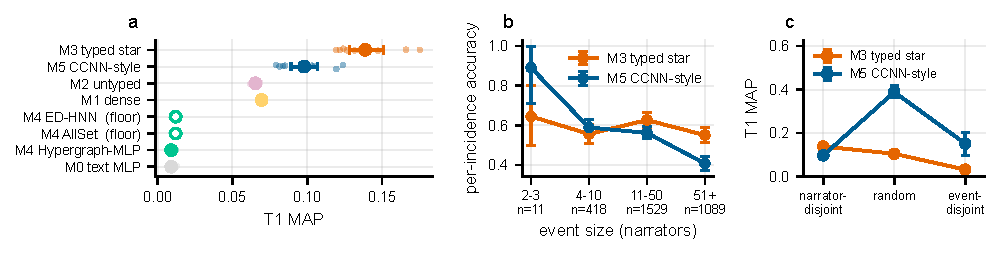
\includegraphics[width=0.72\textwidth]{../figures/fig3_models.pdf}
\caption{The typed star leads at matched budget, its margin widens as events grow, and the
evaluation split decides the ordering. (a) T1 MAP in the primary cell with all ten seeds
shown individually, because means hide bimodality. Hollow markers labelled \emph{floor} are
AllSet and ED-HNN, which never update rank-1 cells, so their T1 values are the frozen-encoder
floor. (b) Per-incidence accuracy stratified by
event size with narrator-clustered 95\% intervals, where $n$ counts held-out incidences.
(c) The same two models under all three splits with everything else held at the
primary cell; both splits that let a narrator appear on both sides of the partition favour
the complex. Intervals in (a) and (c) are bootstrap 95\% CIs over ten seeds, which measure
optimisation noise; the narrator-clustered interval the split claim rests on is in the text.}
\label{fig:models}\label{fig:split}\end{figure*}

\section{Split dependence of the model ordering}

Panel (c) of Figure~\ref{fig:split} was not planned in advance. Under exactly one of the
three splits,
the pre-registered narrator-disjoint one, the typed star leads. Under a random split the ordering inverts and the
complex leads by a wide margin (\MfiveToneRandom{} against \MthreeToneRandom{}). Under an
event-disjoint split it leads again. What those splits share is the partition rather than the
architecture: only the narrator-disjoint split keeps a narrator's segments on one side, so the
other two reward a model for recognising a narrator it was trained on.

The quantity carrying the claim is the difference between those two gaps. Seeds measure
optimisation noise, whereas the sampling unit the claim is about is the query, and queries
cluster by narrator, so we resample \didNarrators{} narrators with replacement over
$10{,}000$ replicates and average over seeds within each. Across those replicates the
complex's random-split gain
exceeds the star's by \didPoint{} MAP, with a 95\% interval of [\didLo{}, \didHi{}]. That
estimate resamples query-bearing narrators and averages inside each replicate, so it does not
equal the difference of the cell means above. Nor does the reversal depend on the selection
rule: reselecting every checkpoint by validation MAP leaves it at \selRandMap{} against
\selRandAuc{} over \selSeeds{} seeds.

Little else matters. Table~\ref{tab:invariance} varies every design axis the field argues
about, granularity, negative-sampling regime and rank map, and the ordering survives
\invarianceWins{} of \invarianceTotal{} conditions. One axis reverses that ordering, and it is
usually a default rather than a decision.

\begin{table}[t]\centering
\caption{The system-level ordering survives every design choice except the split. Each row
varies one
axis with the rest held at the primary cell, and reports how often the typed star leads the
complex on T1 MAP. Every cell uses the star as registered; the input-matched ordering is in
Section~\ref{sec:p3}.}
\label{tab:invariance}
{\footnotesize\setlength{\tabcolsep}{2pt}
\begin{tabular}{lll}
\toprule
design axis varied & levels & typed star leads \\
\midrule
granularity & coarse, mid, fine & 3 / 3 \\
negative sampling & MNS, UNS, SNS, CNS, hard & 5 / 5 \\
rank map & R-A, R-B, R-C & 3 / 3 \\
split & narrator-disjoint, random, event-disjoint & 1 / 3 \\
\bottomrule
\end{tabular}

\vspace{2pt}
{\footnotesize Per-axis counts share the primary cell, so they do not sum: over the 11 distinct cells the typed star leads in 9.}}\end{table}

The random split is a common default, and on this archive the two splits support opposite
conclusions. A model's score under a random split minus its score under an
entity-disjoint one is its \emph{entity exposure gap}, which panel (c) of
Figure~\ref{fig:split} reports per model.

\section{Mechanism: narrator identity in the features}
\label{sec:mechanism}

An explanation is owed, and two experiments run after the split result, labelled exploratory,
supply one more concrete than idiolect. Feature construction is identical for every model: a
rank-0 narrator
is the mean of that narrator's segment embeddings, and a rank-$k$ cell is the mean of its
constituent rank-0 features. Features are built once from the whole archive and split
afterwards, so a narrator's vector aggregates every segment that narrator contributed, and
the narrator-disjoint split closes both routes at once, the repeated vector and the
cross-partition text. Those routes exist because the obstruction of
Proposition~\ref{prop:obstruction} reaches the
features, and that consequence does not depend on this archive.

\begin{proposition}[Lifting carries the obstruction into the features]
\label{prop:singleton}
Let rank-$k$ features be lifted from rank 0 by a permutation-invariant multiset reduction
$\varphi$, so that a cell's input is $\varphi(\{x_s : s \in \mathrm{supp}(c)\})$. Cells sharing
a support share an input, and the distinct rank-1 inputs number at most the distinct supports.
Where a cell has the single owner $\pi(c)$, its input is a function of $\pi(c)$ alone, and
separating two such cells requires message passing through a cell of rank at least two.
\end{proposition}

So \obsCells{} moments admit at most \obsDistinct{} distinct rank-1 inputs, a
\obsCollapse{}-fold collapse (Figure~\ref{fig:overview}b). For the mean, $\varphi(\{x\}) = x$, so a moment's input vector
\emph{is} its narrator's vector; a learnable $\varphi$ changes the value but not the
dependence on $\pi(c)$ alone. We verified the equality: for every narrator holding more than
one such moment, the largest elementwise difference between two of them is exactly zero.

The split decides whether that degeneracy is visible. Of \straddleTotal{} narrators,
\straddleRandomN{} straddle the random split (\straddleRandom{}) and \straddleEventN{} the
event-disjoint one (\straddleEvent{}), since holding out events does not hold out the
narrators who witnessed them. Both place a narrator's vector on both sides of the partition.
A narrator-disjoint split places none. Both rates are predictable before any model exists:
the random split partitions incidences, so assigning a narrator's $k$ of them independently
across folds of proportion $p_f$ predicts
$1 - \sum_f p_f^{k}$, or \exposurePredicted{} against \straddleRandom{} observed, with the
\exposureSingletonN{} single-cell narrators contributing zero. Exposure is not an artefact of
one lifting: across \liftConfigs{} liftings the singleton fraction ranges
\liftSingLo{} to \liftSingHi{} while predicted exposure stays \liftExpLo{} to \liftExpHi{},
because it follows from how many cells an entity owns rather than from how many it owns
alone. Those liftings are this archive's rank maps and granularities, so the sweep bounds the
choice rather than the collection.

That first experiment is easy to over-read, so its control comes first. A linear probe
recovers narrator identity from the \emph{input} rank-1 features at
\probeInputControl{} over \probeClasses{} narrators and \probeN{} moments, against a
majority-class floor of \probeChance{}, a tautology since the classes are identical vectors.
That probe is a multinomial logistic regression over standardised rank-1 vectors, fitted on a
stratified 70/30 split of segments held fixed across seeds and restricted to narrators with at
least four segments; it partitions segments rather than narrators, so every class appears on
both sides.
What the trained models show is how much inherited identity survives
message passing, and the answer is most of it: \probeNarrFive{} for the complex against
\probeNarrThree{} for the typed star under the narrator-disjoint split, \probeRandFive{}
against \probeRandThree{} under the random one. Complex scores are higher in both and the
seed spreads overlap, so neither architecture discards narrator identity.

A second experiment intervenes on the mechanism: we shuffled narrator labels across segments,
preserving segments per narrator, and re-ran both splits. Anonymisation changes which
passages count as positives, so an anonymised score is not comparable to a real one; what is
comparable is the \emph{gap between splits}, because both are transformed alike. With real
narrators the complex gains \gapRealFive{} MAP moving from the narrator-disjoint split to the
random one. With identity destroyed that difference is \gapAnonFive{}, a reduction of
\gapReductionFive{}, so its whole advantage disappears. Its advantage gone, the star's gap
falls too, from
\gapRealThree{} to \gapAnonThree{}, by less than half as far and from a value that was never
positive: the shuffle costs the complex its advantage and costs the star a gap it did not
have.

Shuffling also separates the two routes: it preserves how many segments each label holds, so
cross-partition aggregation survives while identity correspondence does not. That reading
carries a boundary, since a shuffled aggregate has less to leak, so computing features
split-first is the direct test.

Each narrator's vector is rebuilt from that narrator's training-side
segments, a segment counting as training-side when none of that narrator's incidences through
it are held out, with a fallback to a narrator's own segments that is not a leak because a new
interview arrives at deployment with its transcript. Under the random split the
construction strips a mean \sfMeanRemoved{} of the segments contributed by each of
\sfNarrTouched{} affected narrators.

The reversal survives it, which is what we predicted in writing beforehand. Moving from the
narrator-disjoint split to the random one, the complex gains \sfLiftFiveGlobal{} MAP under
global features and \sfLiftFiveSF{} under split-first ones, and the input-matched star gains
\sfLiftThreeGlobal{} and \sfLiftThreeSF{}. Both arms come from one re-run of the primary
cell, so they are comparable to each other rather than to the grid values above.
Removing every token of test-side text leaves the
advantage where it was, so cross-partition aggregation is not the carrier and what the random
split rewards is repeated narrator identity.

The spectral encodings suppress exposure in both architectures, which is the second lever on
the same mechanism. Across the factorial, the star's exposure gap falls from
\facExpThreePlain{} on plain inputs to \facExpThreeEnc{} with the encodings, and the
complex's from \facExpFivePlain{} to \facExpFiveEnc{}. On matched inputs both leak, the
complex by roughly \facExpFivePlain{} against \facExpThreePlain{}, so the leak is
differential rather than present in one architecture and absent in the other. Features that
carry structure rather than identity reduce what a random split can reward, whichever operator
reads them.

\begin{figure*}[t]\centering
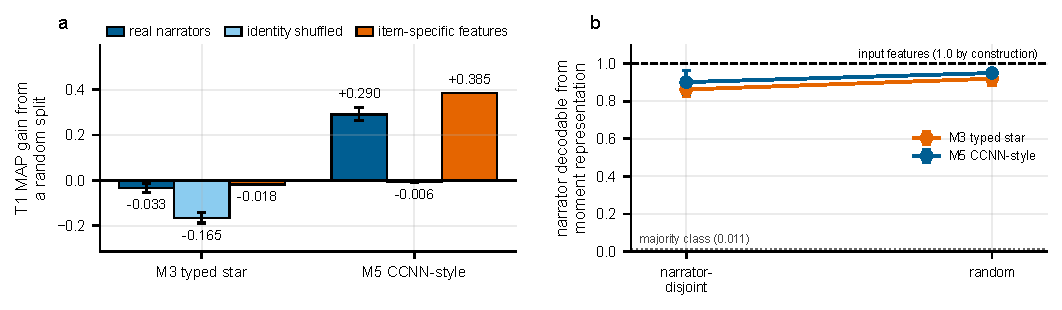
\includegraphics[width=0.77\textwidth]{../figures/fig7_mechanism.pdf}
\caption{Destroying narrator identity removes the complex's random-split advantage, and
editing the moment features does not. (a) Gain in T1 MAP from switching to a random split,
with 95\% intervals over seeds. The item-specific arm was run separately and is measured
against its own baseline, so its bar carries the same quantity but not the same reference as
the other two.
Shuffling narrator labels takes the complex's gain to zero; replacing each moment's vector
with its own passage embedding leaves the gain intact, which locates the leak in the narrator
layer rather than in the moment vector. (b) A linear probe recovering narrator
identity from moment representations, against a majority-class floor of \probeChance{} over
\probeClasses{} narrators. The dashed line is the same probe on the input features,
\probeInputControl{} by construction. The axis runs the full range.}
\label{fig:mechanism}\end{figure*}

The random split does not merely correlate with the complex's advantage: removing what it
leaks removes the advantage. Because a moment is represented by its narrator, a random split
places \emph{the same input vector} on both sides, and the operator that propagates further
through the narrator layer is the one the default split rewards.

A third experiment bounds that account. If the leak were carried by the moment vector alone,
replacing it should close the gap, so we gave every rank-1 cell its own passage embedding
instead of its narrator's mean, holding the complex, the splits, the seeds and the budget
fixed. Two moments by one narrator are then no longer identical at the input, and the gap
still did not close. Against that experiment's own baseline it moved from \featGapMean{} to
\featGapItem{} for the complex, slightly
wider rather than narrower, and the typed star stayed where it was (\featGapMeanThree{}
against \featGapItemThree{}).

We report that as a refuted prediction, because it bounds the claim. Only the rank-1 features
changed; the rank-0 narrator layer and every message path through it stayed in place, and
that is what anonymisation destroys, which is why splitting on the narrator fixes the leak
and editing features does not.

A dose-response prediction is also on the record: the complex's per-narrator random-split
advantage should rise with that narrator's segment count, against a flat control slope. Over
\doseNarrators{} narrators the random-split slope is \doseSlope{} (95\% CI [\doseSlopeLo{},
\doseSlopeHi{}]) against a control slope of \doseSlopeControl{}. That control is not flat: the
complex falls further behind on prolific narrators exactly where it cannot have seen them, so
the mechanism stands on the intervention rather than on the correlation.

Our dense baseline is scored on each passage's own frozen embedding while every trained model
sees its narrator's mean, so \MoneTone{} reflects that trade; the typed star against the
complex, which is what the paper claims, sits on identical inputs.

\section{Four rival explanations}

A negative result is worth reporting only if it survives the obvious explanations. Four were
tested; the segmentation check settles at once, since its three defensible extraction settings
are the granularities of \S\ref{sec:p2} renamed, agreeing no better than \extractorMinRbo{}.

\paragraph{The ordering holds on a cleaned grid.} The event layer is
under-merged (\S\ref{sec:extractor}), so perhaps the complex is being asked to model damage.
Rebuilding the archive with the \goldTermsExcluded{} contested terms removed leaves
\goldSubsetSegments{} segments and \goldCells{} rank-2 cells, against the \nRankTwoCells{}
the primary complex carries. All models rise on the reduced grid because the candidate pool
shrinks. On that grid the star--complex ordering is unchanged, \goldMthree{} against
\goldMfive{}, so the
complex is not being asked to model damage. A parameter-free baseline rises furthest, to
\goldMone{}, and overtakes both, which is a pool-size effect and a reminder of how little of
this ranking the learned structure contributes.

\paragraph{Curated cells survive their own error rates.} We propagated the measured merge and
split error rates through the complex over a \pertGridPoints{}-point grid per calibration,
twenty draws each. Calibrated to the archive's internal disagreement, the triage list retains
$\text{RBO}_{50} = \pertRboArchive{}$ against the unperturbed ranking, clear of the registered
threshold of \pertThreshold{}, and that is the figure governing the triage we report, since
the complex analysed here is built from the curated vocabulary. Substituting the automatic
extractor's own error rate drops retention to \pertRbo{}, below the threshold, whose committed
consequence is that an automatically built triage list is a screening step needing human
verification. Instability here is inherited from the extractor, not from the curated cells.

\paragraph{Counting interviewers erases the phenomenon.} Counting interviewer turns as
attestations would inflate every cell: the singleton fraction
falls from \singletonNarrators{} over narrators to \singletonWithInterviewers{} once
interviewers count, because an interviewer is present in every segment, so every event
acquires a second voice and nothing is under-attested. Both triage lists still agree at
\interviewerRbo{}, which is why the decision looks harmless until the quantity that matters
is inspected.

\section{Utility of the representation}

The application claim is archival triage: surfacing events that rest on too few voices. The
quantity ranked is \emph{archive-conditioned} attestation multiplicity, how many narrators
\emph{in this collection} describe an event, so an event thinly attested here may be
abundantly documented elsewhere, and it presupposes curation, since rank-2 cells come
from the
archive's controlled vocabulary. Two questions decide whether the machinery earns its place.

\paragraph{A minority of triage items are unstable under resampling.} Of the top \triageK{}
triage items, \triageUnstable{} are unstable under the conditions tested. The list is a
screening device, and each item ships with the probability that it is a singleton only
because of extraction error.

\paragraph{Mention frequency sets the bar the structure has to clear.} Archive-conditioned attestation
multiplicity correlates with bare mention frequency at $\rho = \freqSpearman{}$, the two
triage lists agree at $\text{RBO}_{50} = \freqRbo{}$, and they share a Jaccard overlap of
\freqJaccard{} in their top ten. Counting mentions recovers most of what the ladder, the
encodings and the complex were built to recover, so the structure-derived ranking has to
justify itself where the two disagree, and that region is the minority of the list.

\section{Transfer to a held-out collection}

What transfers is a conclusion rather than a model: every threshold, rank map
and hyperparameter was applied as fixed on the primary archive, with no tuning, to
held-out
collections of \transferInterviews{} interviews and \transferSegments{} segments. Rank and
cardinality: $\rho = \transferRho{}$ over \transferCells{} rank-2 cells. Rank agreement:
$\alpha = \transferAlpha{}$. Models: typed star \transferMthree{}, complex
\transferMfive{}. Those levels are not comparable with the primary archive's, since this
collection carries \transferCells{} rank-2 cells against \nRankTwoCells{} at home and has no
transcripts, so we leave the model comparison unread there. Our
pre-registered test is narrower: whether the interaction estimate keeps its sign and
magnitude. It does not, so the interaction finding is archive-specific, as we committed in
advance.

\section{Release and instruments}

A registered topology analysis is absent, and the reason generalises: its permutation null
tests nothing, since shuffling which
rank-2 cell holds which narrator set is a relabelling and homology ignores labels, so
$p = \topoPermP{}$ was forced by construction. Event-size and connectivity moments predict
$\beta_1$ at $R^2 = \topoBetaOneRtwo{}$, above the registered $0.9$, so the verdict is
\topoKeep{}.

Every estimator was asserted against a known answer before being pointed at the archive,
which caught eight defects that would otherwise have been reported as findings, among them a
link task whose message passing was handed the edges it had to predict. Every
reference was retrieved programmatically and accepted on a title match above $0.92$ with
the first author confirmed. Our release, \emph{CAIRN} (\url{\repoURL}), is stand-off because
the archive's
material is not ours to redistribute, and carries the cell definitions, incidence matrices at
all three granularities, the splits, the annotation manual, a licence audit, the defect log,
the substitution record and a fetch script.
A fresh interpreter recomputes the headline corpus statistics from those files alone, which is
the reproduction the release supports; independent human replication is the one substitution
still outstanding.

\section{Limitations}

Six substitutions are on the record, each bounding the claim in a stated direction. The
agreement study measures whether the manual determines the assignment rather than whether
people agree, and the transfer collection refutes a strong effect without confirming a weak
one. Four others are registered: no expert panel, no external coreference corpus, no second
archive, and a self-sufficiency check for independent reproduction. No contemporary
generalised-CCNN baseline was run, so the operator comparison is with the star expansion and
the hypergraph family rather than with that line. Our corpus is one archive
in one language, and the ladder is its cataloguers' choice, so a different descriptive
tradition could behave differently. What survives those caveats is the structure of the
argument: the three preconditions are testable anywhere, and the lifting creates the same
exposure wherever cells share recurring owners, though the magnitude and the reversal are
findings on this archive.

\section{Conclusion}

The ownership obstruction is what this archive turned up. Where items are singly owned, the
cells above the owners are not subsets a combinatorial complex can hold apart, and here
\obsCells{} moments collapse onto \obsDistinct{} supports, so a lifted rank-1 feature is a
function of who owns it. Rank carries information beyond cell cardinality and the star
expansion is lossless, so the ladder is real; the specification does not yet supply a
reproducible assignment, and the complex has still to earn its extra structure. What the star
wins with, though, is its inputs: on matched features the ordering reverses, so the
registered verdict is about the system rather than the operator.

Evaluation decides whether the collapse is visible. A random split lifts the complex
\didPoint{} MAP more than it lifts the star (95\% CI [\didLo{}, \didHi{}]), and that
difference survives rebuilding every feature split-first, so the carrier is repeated narrator
identity. Shuffling that identity removes the advantage, and giving each moment its own
passage text does not. Beyond this archive, the obstruction reaches any collection whose
items belong to recurring
entities, so the defence is to split on the entity, and to check what a rank-1 cell contains
before concluding that rank helped.

\bibliographystyle{IEEEtranN}
\bibliography{references}
\end{document}
